\subsection{Presentation interface}

The concept of this interface is to keep the user from accessing their devices, just to check to current playlist configuration but instead provide quick and easely accessicible overview for the users of the system, bargoers and administrator both. By having seperated screen from the users devices, the system may reduce the amount of time spent using the devices which was declared a problem, best seen minimized, as an effect of the system, concluded in \cref{sub:user_requirements}. \chnote{måske noget deb teori om at man kigge op instedet for ned på en telefon, har en positiv effect, husk find kilde!}
This is a part of the system which always visually accessible for the user, therefore should also be visually pleasing to look at, \chnote{Kom med noget bullshit om deb, måske google material guiden}. \cref{fig:PresentationInterface} is a sketch of the screen in context and visual design. \chnote{skift billed}

\begin{figure}[H]
  \centering
  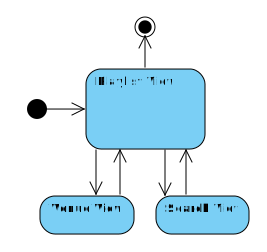
\includegraphics[width=1.0\linewidth]{Images/UserInterface.pdf}
  \caption{Sketch of the screen in context and visual design}\label{fig:PresentationInterface}
\end{figure}